\chapter{Loop Closures using an Omni Camera}
\label{chapter:omni_loop_close}

\section{Place Recognition}

The first step is to substitute omni camera images in the place recognition module. The donut image format is not preferred for the place recognition.  They contains blind spots (inner and outer circle), which contain some texture, and are also susceptible to change from internal reflections within the lense.  In terms of place recognition, this would add noise to each image and therefore the unwrapped image is preferred.

It is computational expensive to unwrap every frame, this would mean processing 1280x960 images at 30Hz.  This would also introduce complications in synchronizing stereo frames with omni frames.  Therefore only keyframe images are unwrapped.  A omni camera image buffer records a short history of donut image frames.  When a new keyframe is created, the timestamp of the stereo image used for this keyframe is sent to the buffer object, which finds the corresponding omni camera image and unwraps it.  This unwrapped image is saved with the keyframe and sent to the place recognition module.  This reduces computational cost and simplifies omni-stereo synchronization.

As described in section \ref{sec:bag_of_words}, the place recognition system employs clustering of detected SURF features in feature space using a bag of words approach.  This means that in the case of $360^\circ$ circular images, it will be invariant to rotation about the upward facing axis, as the locations of 2D features are not considered.  This is ideal for this particular use case.

\section{Calculating transformations for loop closures}
\label{sec:calc_loop_edge}

A match from the place recognition module itself is not enough to do a global loop closure.  As described in section \ref{sec:scavislam_place_recog}, a geometry check is required to filter false positive matches and determine a metric rigid body transformation so the loop closure may be added to the graph.

It has also been mentioned in section \ref{subsec:selected_approach} that calculating a transformation using a monocular camera such as the omni camera introduces the arbitrary scale issue.  (For further explanation of the scale issue, see Chapter \ref{chapter:MultiCamSLAM}). Therefore the stereo information needs to be combined with the omni camera in order to produce a metric scale transformation.  Two methods were developed to address this scale issue, a 'scale correction' algorithm, and using the p3p algorithm.  These methods will be discussed in detail in the following sections.

\subsection{Scale Correction algorithm}

The main idea behind this algorithm is a two stage approach, first calculate the non-metric transformation using images from the omni camera and then correct it to metric scale using stereo data.  An important consideration is that the omni camera will find loop closures where stereo wouldn't, so one must assume that there will be likely zero overlap between stereo poses, and therefore no feature matching possible between these two frames. (see fig \ref{fig:omni_loop_close})

\subsubsection{Pose estimation}

First step is to calculate a non metric transformation using the two omni frames only.  This is done using the 5 point algorithm as mentioned in section \ref{subsec:5point}.  This returns a non metric pose and a set of inlier points used to calculate this pose, represented as 3D vectors (also non metric scale).

\subsubsection{Scale Offset Calculation}

Points with metric scale are calculated using stereo matching.  These points are then matched to feature points from the omni camera images and compared with 3D non metric points returned from the pose estimation.  A scale offset is calculated per point.  (fig.\ref{fig:scale_offset}) The pipeline that calculates a list of scale offsets is listed below, and represented in fig \ref{fig:scale_adjust_flowchart}.  This pipeline takes left, right and omni images as an input, and may be applied to either of the two loop closure frames separately.  In practice both frames are used and the scale list are concatenated together.

\begin{figure}[h]
  \centering
  \begin{align}
   S =
   \displaystyle\frac{
   \left|\displaystyle\frac{\bv {MP}_{x}}{\bv P_{x}}\right| + 
   \left|\displaystyle\frac{\bv {MP}_{y}}{\bv P_{y}}\right| + 
   \left|\displaystyle\frac{\bv {MP}_{z}}{\bv P_{z}}\right|
   }
   {3}
  \end{align}
  \caption{Scale calculation for a single point.  $\bv{MP}$ denotes the metric 3D point calculated from stereo and $\bv{P}$ denotes the non metric 3D point used in pose estimation}
  \label{fig:scale_offset}
\end{figure}

\begin{enumerate}
\itemsep0em
 \item Perform circular matching between left/right/omni images %TODO screenshot
 \item Triangulate 3D points in metric scale using left/right stereo circular matches
 \item For each 3D stereo point:
 \begin{enumerate}
   \item Ensure the matching omni point was an inlier used in pose estimation
   \item Obtain the 3D non metric point triangulated from 5-point transform
   \item Transform the stereo point to the omni camera frame from the extrinsic calibration $\bv P_{om} =  ^{om}\bv T_{st} \bv P_{st}$
   \item Calculate scale offset as per formula \ref{fig:scale_offset} %TODO
   \item Add to list of offsets 
 \end{enumerate}
\end{enumerate} 

\begin{figure}[H]
  \centering
    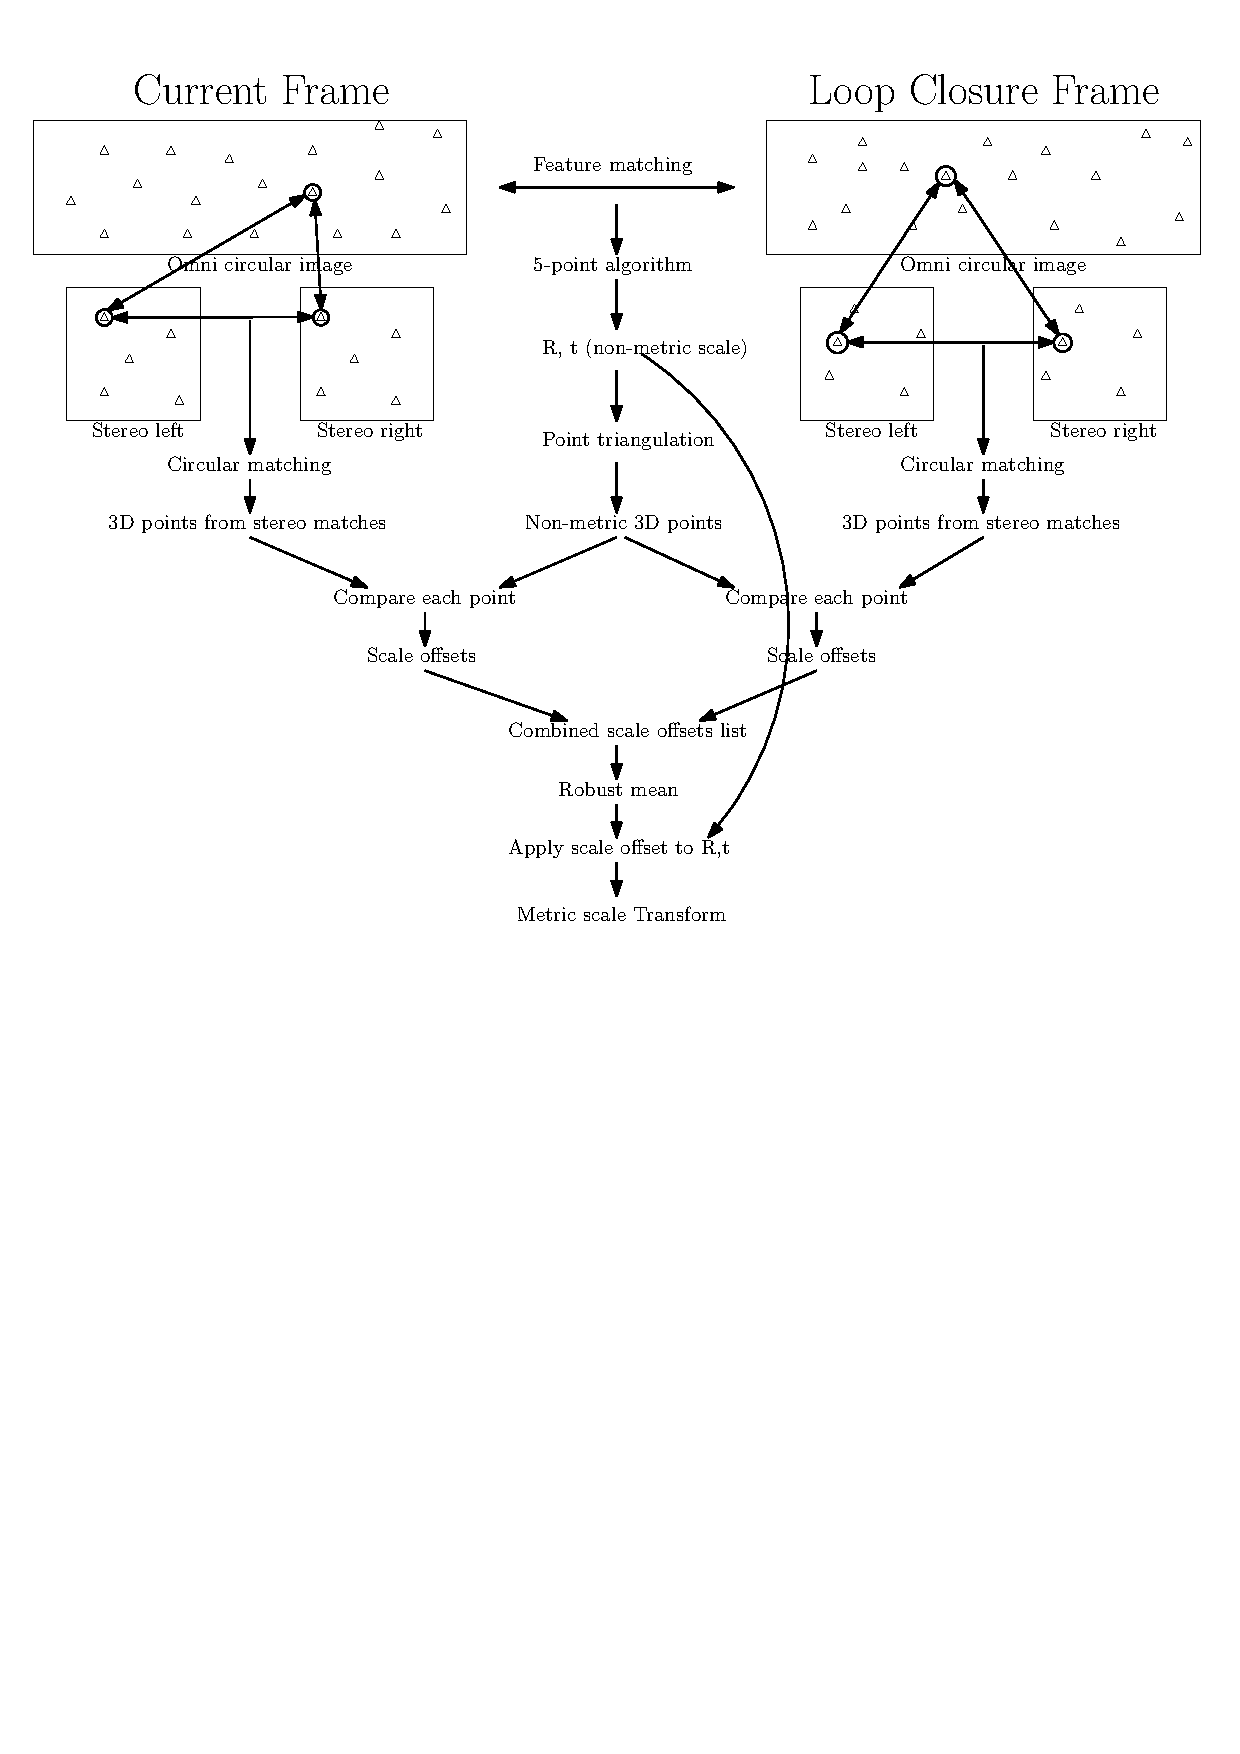
\includegraphics[width=1.0\textwidth]{chapters/images/6_images_scale_adjust}\\
  \caption{Outline of the scale adjustment pipeline}
  \label{fig:scale_adjust_flowchart}
\end{figure}

\begin{figure}[H]
  \centering
    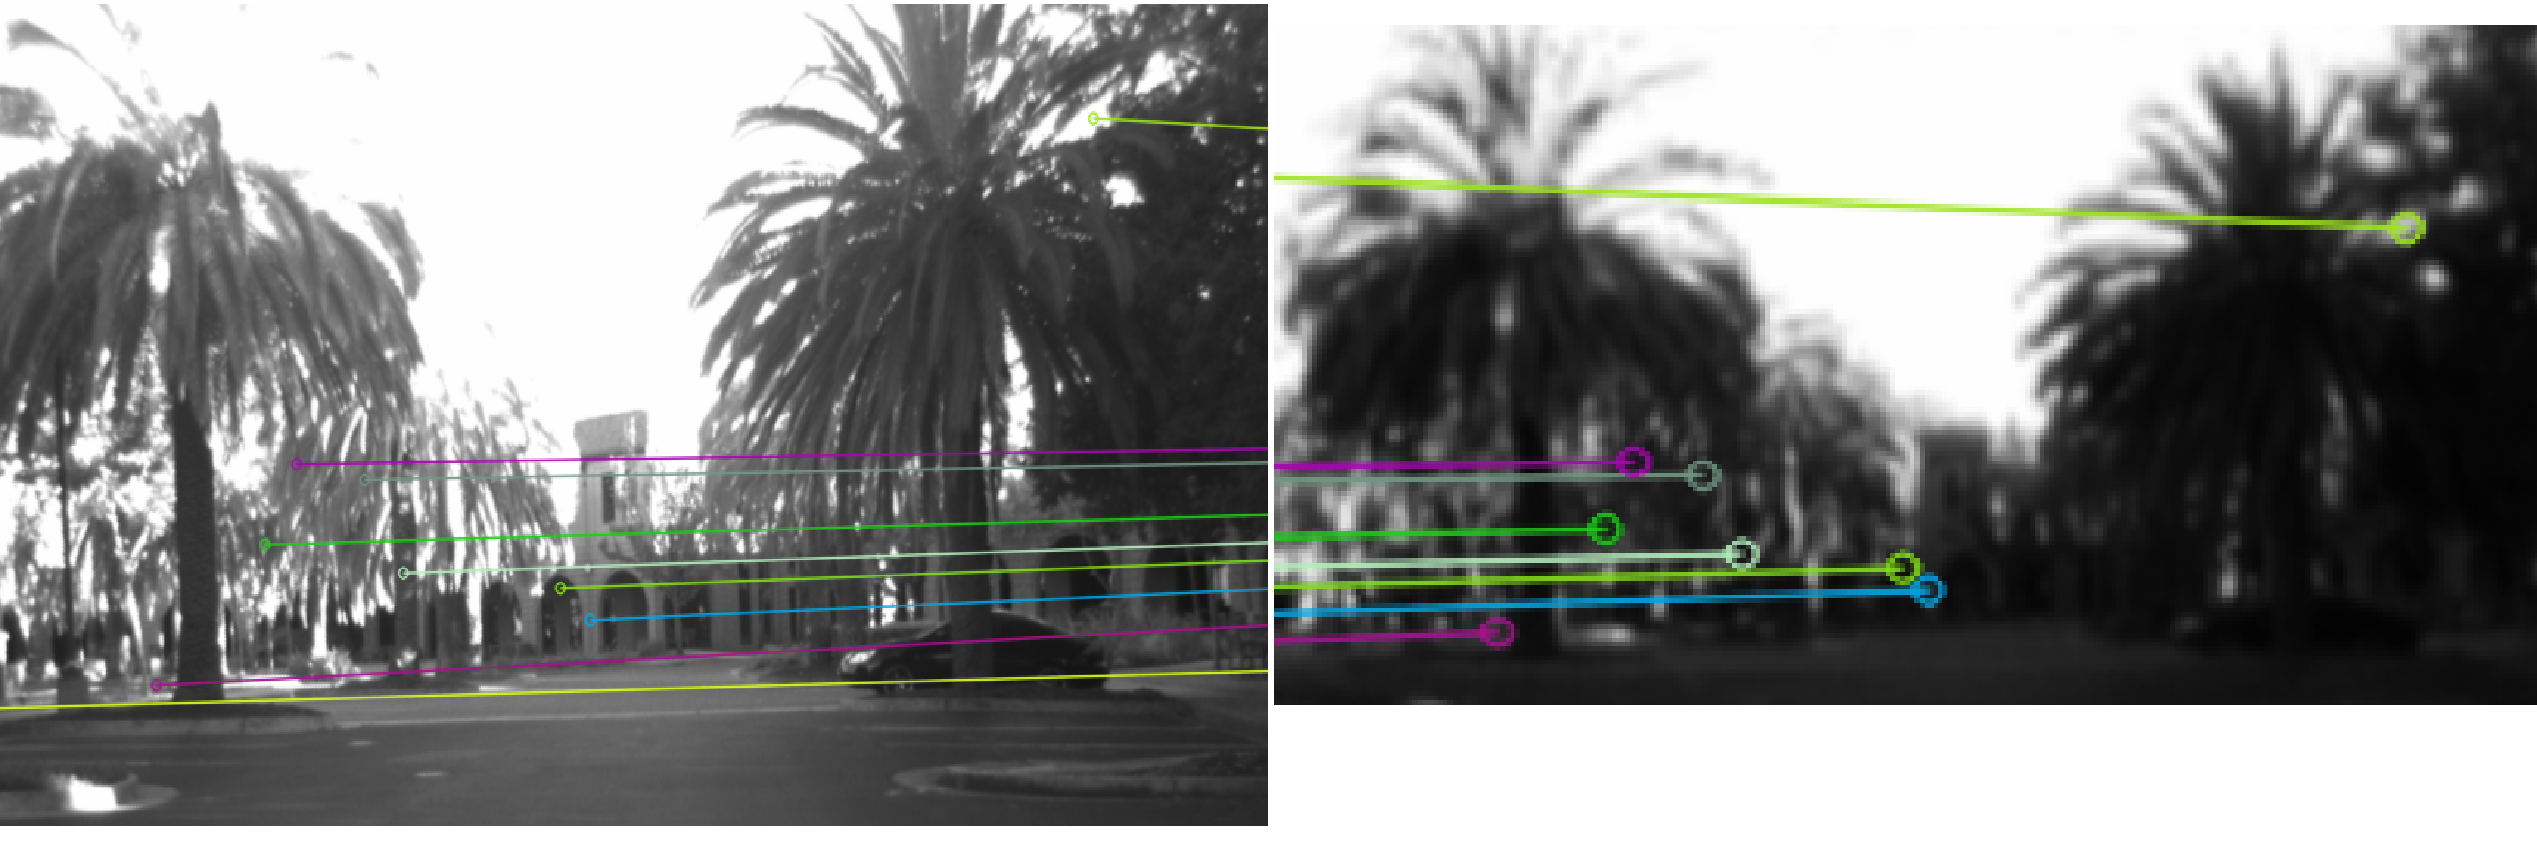
\includegraphics[width=0.8\textwidth]{chapters/images/circular_match}\\
  \caption{Results of circular matching between left, right and omni frames. Left is one of the stereo images and right is a cropped part of the unwrapped omni image. The circular matching produces robust matches without having strict SIFT matching thresholds}
  \label{fig:circular_match}
\end{figure}


%TODO visualization of scale offsets

%TODO visualization of 180 deg pose: slides from last intern meeting

\subsubsection{Robust scale estimation}

Having determined a number of scale offsets, a single offset needs to be determined.  It is likely that outliers exist in the data and these need to be considered.  A potential approach would be to apply RANSAC, choosing a single point and scaling the values and comparing them to their correspondences.  A simpler and less computationally expensive method would be to calculate a robust mean.  A robust mean is calculated in this case using some dude's robust mean algorithm (citation).

%TODO robust mean citation

\begin{figure}[H]
  \centering
    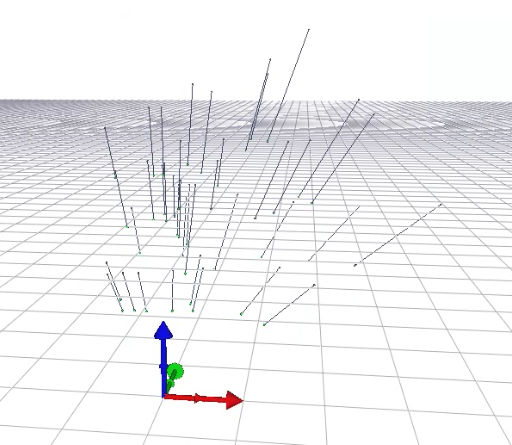
\includegraphics[width=0.6\textwidth]{chapters/images/scale_matches}\\
  \caption{Visualization of non metric points and their corresponding metric scale matches}
  \label{fig:circular_match}
\end{figure}

\subsection{p3p Implementation}

As opposed to the two step approach described above, this implementation calculates a metric transformation using stereo and omni camera data in one step.

The p3p algorithm (cite, section \ref{subsec:p3p}) calculates a transformation between frames given a set of 2D to 3D correspondences.  The scale of the transformation is propagated from the 3D points.  This means after triangulating the new 2D points with the transformation obtained, they will be to the same scale as the existing map.

In this case this algorithm could be used the following way:

\begin{enumerate}
\itemsep0em
 \item Perform circular matching between left/right images from one keyframe, and omni image from the other keyframe
 \item Triangulate 3D points in metric scale using left/right stereo circular matches
 \item Use p3p algorithm; correspondences are known between 3D stereo points and 2D omni points
\end{enumerate}

\begin{figure}[H]
  \centering
    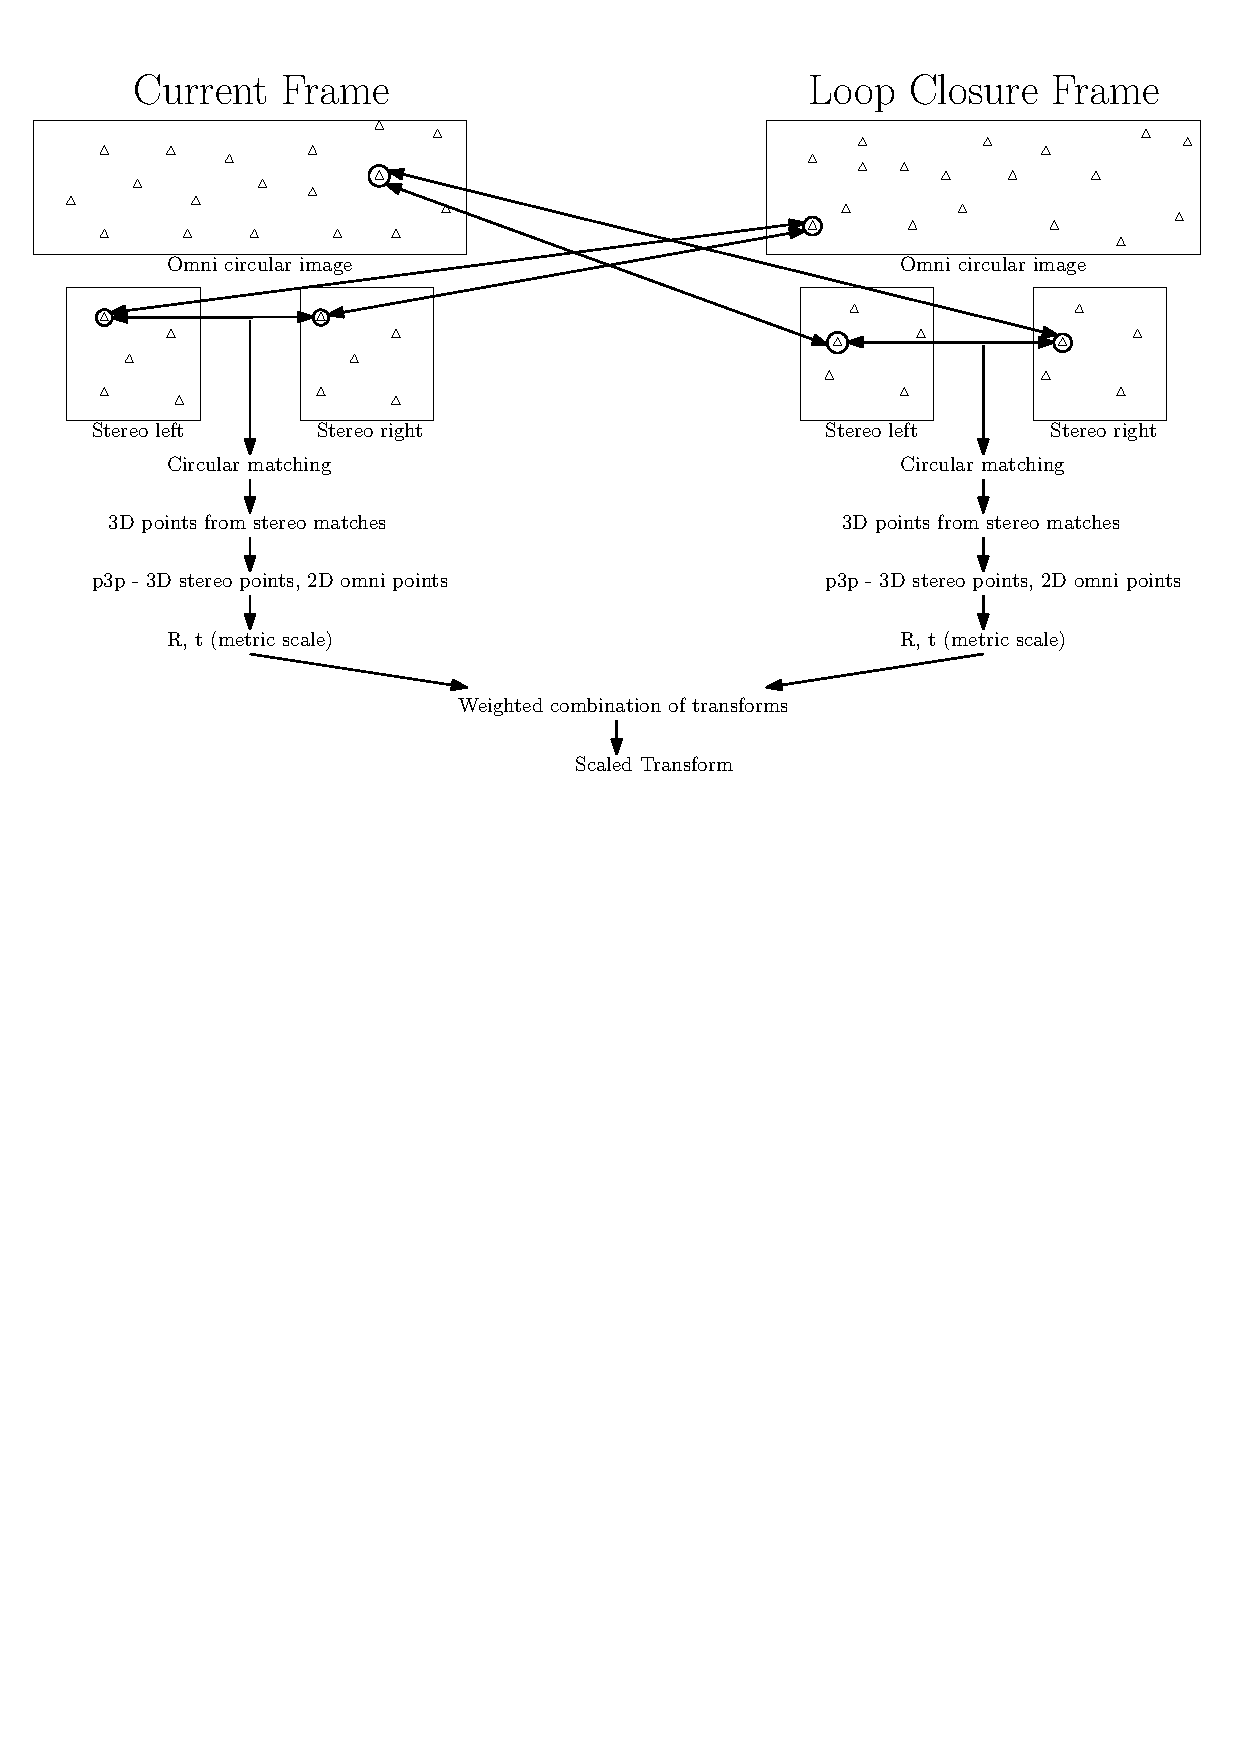
\includegraphics[width=1.0\textwidth]{chapters/images/6_images_p3p}\\
  \caption{Outline of the p3p based pipeline}
  \label{fig:p3p_flowchart}
\end{figure}

This will directly calculate a pose between the two keyframes to the correct scale.  It can also be run twice, matching stereo and omni in both directions. In terms of implementation this is a much neater solution, and would be preferred.  However there are a few pitfalls why it was not chosen as the solution to evaluate on.

\subsection{Comparing methods}

In practice the p3p turns out to be not as accurate as the scale adjustment algorithm.  The number of matches between the stereo camera and the omni camera of the other keyframe is typically very low.  Not only is matching occuring between different cameras, resulting in differing scale and intensities of feature patches, but there is also a larger translation between cameras. Whilst in the scale correction algorithm, these matches are only used for scale adjustment, in the p3p pipeline they are used for pose estimation.  Scale adjustment only requires 1 correspondence, however pose estimation requires 3.  There are likely to be outliers and therefore desirably a multiple of the minimal number of correspondences is needed to determine a good pose.

The scale adjustment algorithm uses all the matches between two omni poses to calculate a transform.  In later evaluations this is shown to be typically well over 100 inliers for pose estimation.  This results in a highly accurate transformation.  The rotation part of the transform does not need to be scaled and can be used directly.  As stated above, only one point is required to determine the scale offset so scale adjustment should be accurate even with few matches.

Finally another advantage of the scale adjustment algorithm is the way in which the data from both frames is fused.  For both algorithms, they can be run twice using first one keyframe, and then the other. (see fig. \ref{fig:scale_adjust_flowchart} and fig. \ref{fig:p3p_flowchart})  Whilst the scale adjustment algorithm outputs two offset vectors that can easily be combined to determine a single robust offset value, the p3p implementation generates two separate poses that need to be fused together somehow.  They could be averaged or both added to the graph weighted on the number of inliers. Nevertheless incorporating all available data into calculating one transform should achieve better results than calculating two not as accurate poses and averaging them together.

\begin{figure}[H]
  \centering
    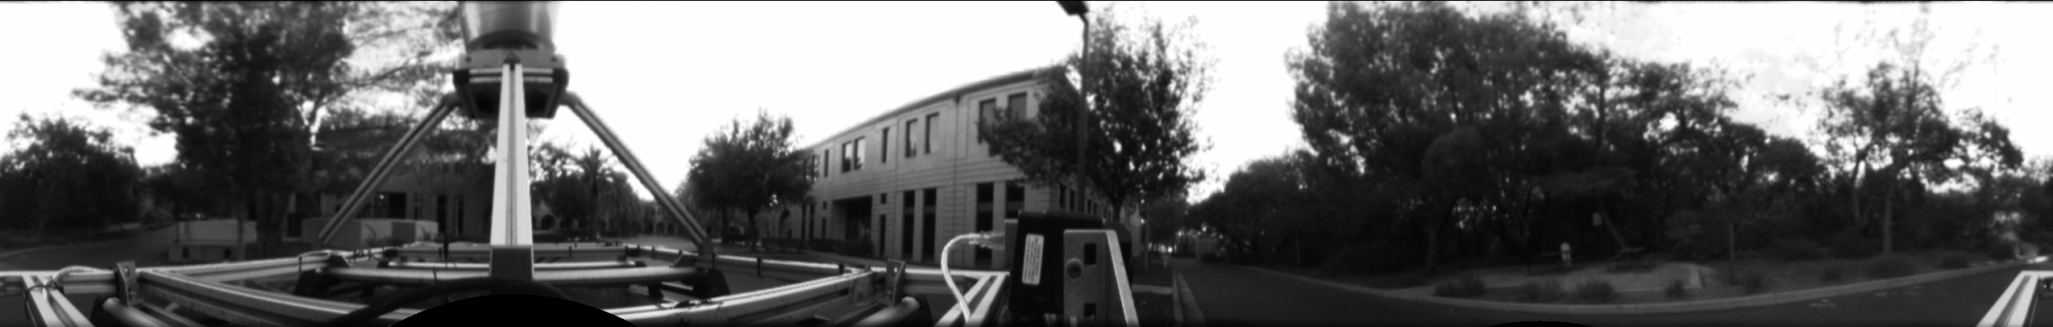
\includegraphics[width=1.0\textwidth]{chapters/images/omni_source}\\
    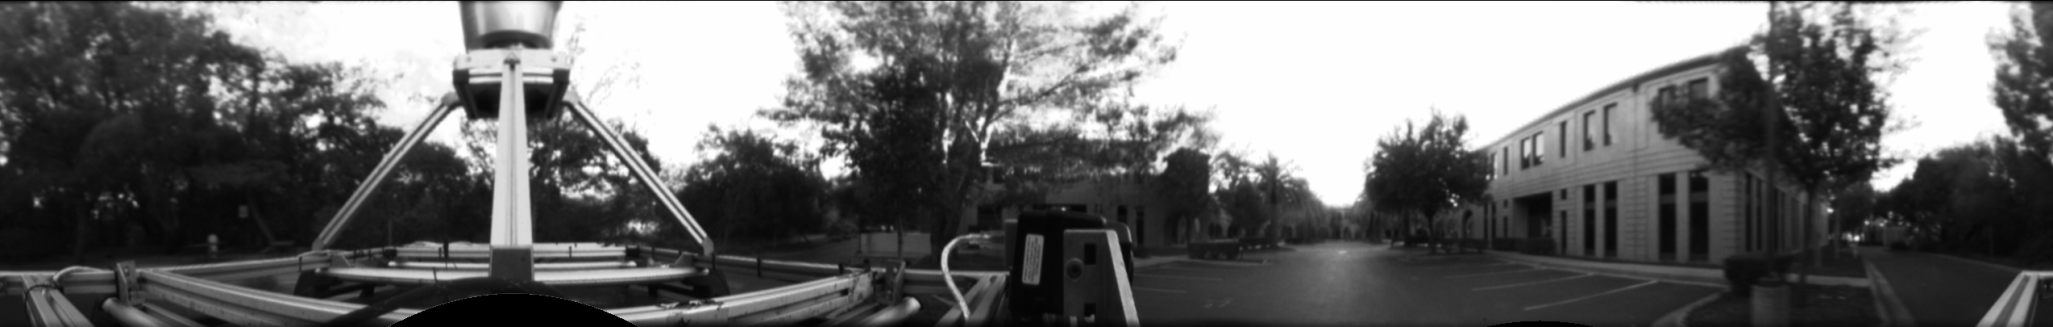
\includegraphics[width=1.0\textwidth]{chapters/images/omni_target}\\
    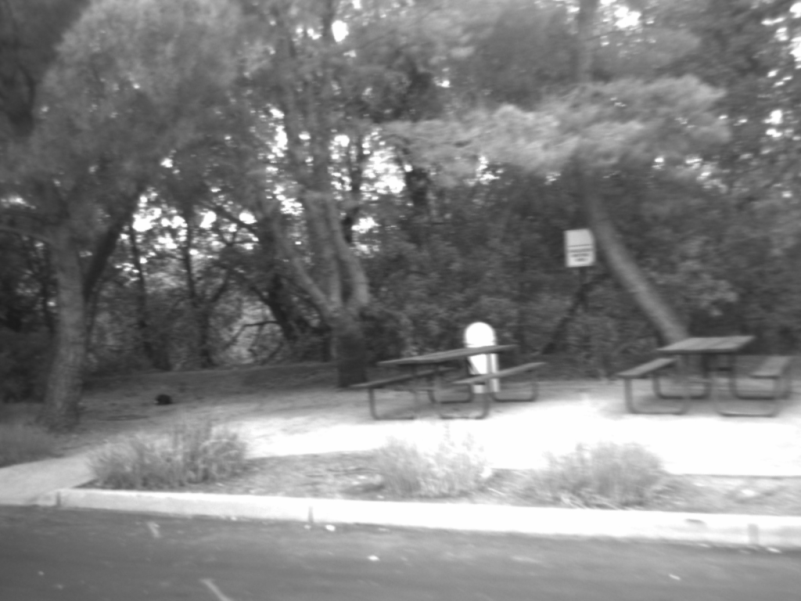
\includegraphics[width=0.49\textwidth]{chapters/images/stereo_source}
    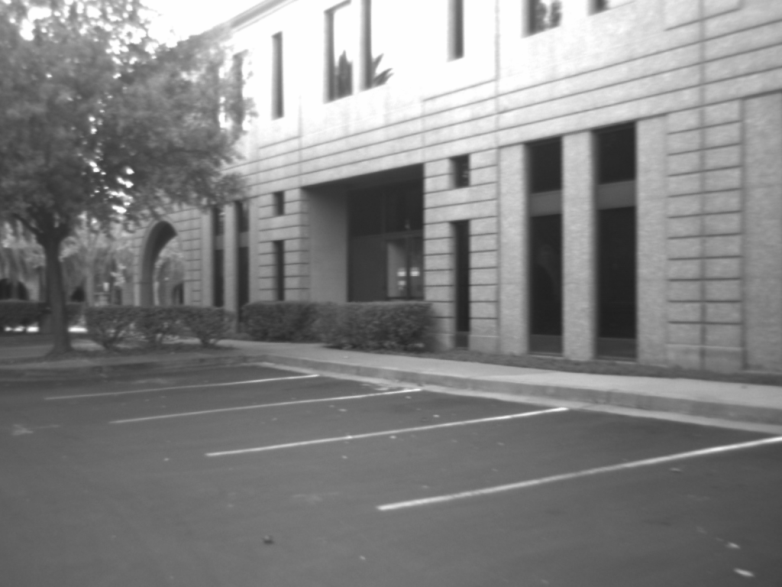
\includegraphics[width=0.49\textwidth]{chapters/images/stereo_target}\\
    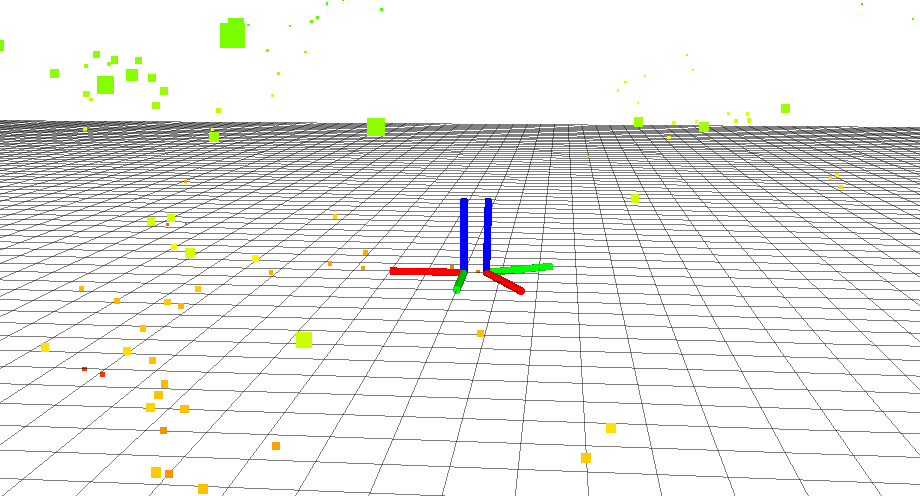
\includegraphics[width=1.0\textwidth]{chapters/images/loop_closure_pose}
  \caption{Example of a pose invariant loop closure using scale adjustment algorithm.  Top shows the two omni images.  Middle shows what the stereo camera sees from these poses.  There is clearly no overlap in the stereo frames.  Bottom shows the metric transformation visualized as a pose, along with 3D pose inlier points in metric scale.}
  \label{fig:}
\end{figure}
\section{Introducing loop closure constraints to the SLAM graph}

Having obtained a transformation between frames, this needs to be integrated into the SLAM graph somehow.  This is not so trivial, especially given that the ScaViSLAM graph utilises the double window approach.  (Sec. \ref{sec:scavislam_graph}).  This section outlines how an edge was added to the graph.

\subsection{Bundle Adjustment vs Pose-Pose edge}

Section \ref{sec:calc_loop_edge} describes returning a single SE(3) edge constraint between keyframes.  This edge can easily be added to the graph.  It would also be just as valid for the pipeline to provide 3D landmarks and shared observations as an output.  In this case the 3D landmarks would be added to the graph as vertices and the shared observations would be added as reprojection edge constraints.  The graph optimization would then calculate the relative pose constraint based on all shared observations, as per a typical bundle adjustment.  The advantage of this is that it more accurately represents the constraint between keyframes than an SE(3) edge  with an estimated information matrix.  In addition, this would work well for the p3p pipeline, as it would solve the problem of how to combine two separate transformations.  Using this representation, consecutive loop closures could add even more observations to existing landmarks to further refine the poses.  However, in order to achieve this, the data association for all landmarks would need to be handled.  This essentially means building a whole new SLAM system, which is out of the scope of this work.

Given that no data association will be done between multiple loop closures, there is little advantage of calculating the constraint using bundle adjustment.  Calculating a keyframe pose-pose edge and estimating the information matrix closely approximates the constraint and is also far more computationally efficient.  Finally, implementing the bundle adjustment, accounting for the double window approach would also be considerably more effort than SE(3) edges.

%\subsection{Adding the pose to the inner window}

%The place recognition module will return potential loop closures for the most recently added keyframe.  If a loop closure is successful, this means it will connect to a keyframe in the inner window.  However adding a single edge to the inner window will have little affect, as there will be too many landmark observation constraints opposing this edge.  If the stiffness of the new constraint is set high enough, the particular keyframe will be pulled towards the direction of the loop closure, but all the other keyframes will remain in place. (fig. \ref{fig:graph_fail})

%\begin{figure}[H]
%  \centering
%    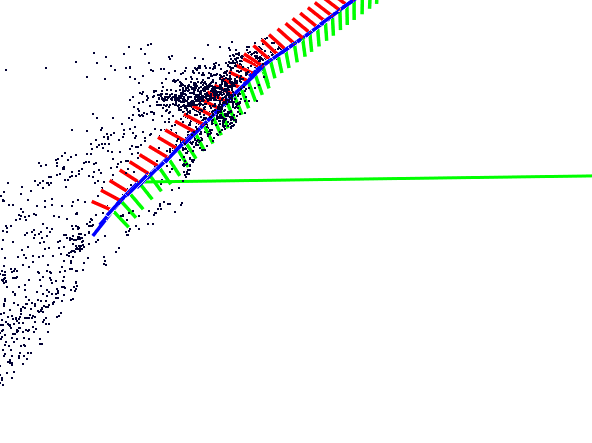
\includegraphics[width=0.49\textwidth]{chapters/images/before_opt}
%    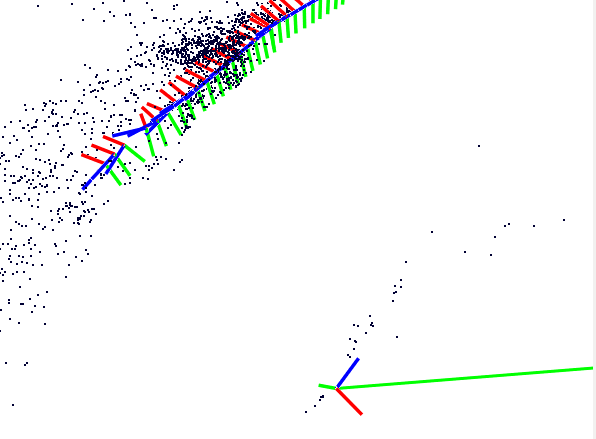
\includegraphics[width=0.49\textwidth]{chapters/images/after_opt}
%  \caption{Adding a SE(3) edge to the inner window.  Black dots denote landmarks.  The green line is the SE(3) loop closure edge}
%  \label{fig:graph_fail}
%\end{figure}

%In order to deal with this problem, after adding a loop closure edge, the graph is 'reinitialised' to a new configuration using SE(3) edge only optimization.  The entire inner window is marginalised to SE(3) edges, as they would be when leaving the inner window.  This is essentially the same as changing the inner window size to 1.  Then optimization is performed, this time with the loop closure edge having a more equal weighting to the rest of the constraints.  The graph error is then spread evenly throughout the graph, and the current pose is moved to the loop closure keyframe.  Having completed this optimization, the inner window is restored and the graph retains its structure.

%\begin{figure}[H]
%  \centering
%    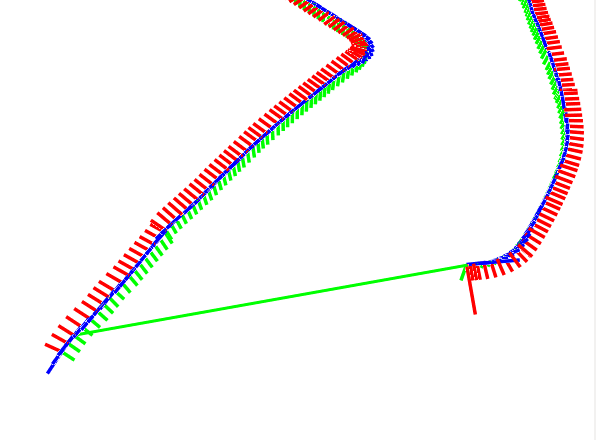
\includegraphics[width=0.45\textwidth]{chapters/images/before_opt_good}
%    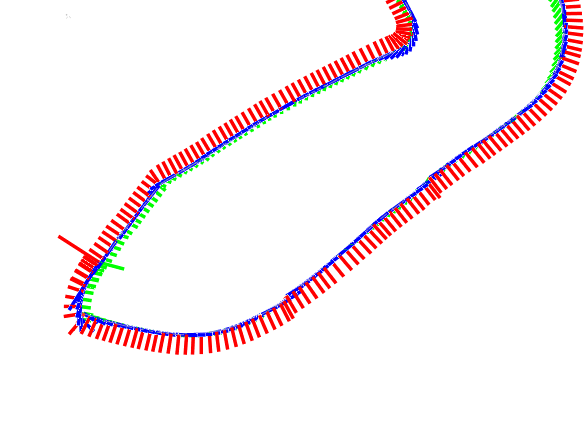
\includegraphics[width=0.45\textwidth]{chapters/images/after_opt_good}
%  \caption{Before and after optimization using pose only constraints}
%  \label{fig:graph_fail}
%\end{figure}